%% ==============================
\chapter{\iflanguage{ngerman}{Ergebnisse}{Results}}
\label{sec:results}
%% ==============================
\section{Experimental Setup for Evaluation}
Network card : lshw command
cpu : lscpu
memory: sudo dmidecode --type 17

\begin{table}[htbp]
    \centering
\begin{tabular}{ |c|c|c|c| }
\hline
\multicolumn{4}{|c|}{Overview of PCs used for the evaluation} \\
\hline
& PC1 & PC2 & PC3  \\
\hline
\hline
\textbf{Hardware} &  &  & \\\hline
    Processor &
        \begin{minipage}{3.9cm}
	       \vskip 8pt
		      16 $\times$ AMD Ryzen 7 5800H with Radeon Graphics
	       \vskip 8pt
	    \end{minipage} & 
        \begin{minipage}{3.9cm}
    	    \vskip 8pt
    		   16 $\times$ AMD Ryzen 7 5800H with Radeon Graphics
    	    \vskip 8pt
	    \end{minipage} & 
        \begin{minipage}{3.9cm}
	       \vskip 8pt
		      16 $\times$ AMD Ryzen 7 5800H with Radeon Graphics
	       \vskip 8pt
	    \end{minipage} \\\hline
    RAM &
        \begin{minipage}{3.9cm}
	       \vskip 8pt
		      2 $\times$ 32GB DDR4 Samsung SODIMM 3200 MT/s
	       \vskip 8pt
	    \end{minipage} & 
        \begin{minipage}{3.9cm}
    	    \vskip 8pt
    		   2 $\times$ 32GB DDR4 Samsung SODIMM 3200 MT/s
    	    \vskip 8pt
	    \end{minipage} & 
        \begin{minipage}{3.9cm}
	       \vskip 8pt
		      2 $\times$ 32GB DDR4 Samsung SODIMM 3200 MT/s
	       \vskip 8pt
	    \end{minipage} \\\hline
    Network Card &
        \begin{minipage}{3.9cm}
	       \vskip 8pt
		      Realtek Semiconductor Co., LtdRTL8125 2.5GbE Controller
	       \vskip 8pt
	    \end{minipage} & 
        \begin{minipage}{3.9cm}
    	    \vskip 8pt
    		   Realtek Semiconductor Co., LtdRTL8125 2.5GbE Controller
    	    \vskip 8pt
	    \end{minipage} & 
        \begin{minipage}{3.9cm}
          \vskip 8pt
		      Realtek Semiconductor Co., LtdRTL8125 2.5GbE Controller
	       \vskip 8pt
	    \end{minipage} \\\hline\hline
\textbf{Setup} & & & \\\hline
    Operating System & Kubuntu 22.04 &  Ubuntu 22.04 & Ubuntu 22.04 \\\hline
    Kernel &
        \begin{minipage}{3.9cm}
	       \vskip 8pt
		      A
	       \vskip 8pt
	    \end{minipage} & 
        \begin{minipage}{3.9cm}
    	   \vskip 8pt
    		   B
    	   \vskip 8pt
	    \end{minipage} & 
        \begin{minipage}{3.9cm}
	       \vskip 8pt
		      C
	       \vskip 8pt
	    \end{minipage} \\\hline
    Real-time Kernel &
        \begin{minipage}{3.9cm}
	       \vskip 8pt
    		   A
    	   \vskip 8pt
	    \end{minipage} & 
        \begin{minipage}{3.9cm}
    	   \vskip 8pt
    		   B
    	   \vskip 8pt
	    \end{minipage} & 
        \begin{minipage}{3.9cm}
    	   \vskip 8pt
    		   C
    	   \vskip 8pt
	    \end{minipage} \\\hline
    ROS version & Rolling & Rolling & Rolling \\\hline
        \begin{minipage}{3cm}
        \vskip 4pt
    		   ros2\_control based on commit:\vskip 8pt
	    \end{minipage} & 0eb319ea43b78b886a & 0eb319ea43b78b886a & 0eb319ea43b78b886a \\\hline
            \begin{minipage}{3cm}
        \vskip 4pt
    		   ros2\_controllers based on commit:\vskip 8pt
	    \end{minipage} & 05d7a5ec73a02eab2c & 05d7a5ec73a02eab2c & 05d7a5ec73a02eab2c \\\hline
\end{tabular}
    \caption{Three different computers were used for the evaluation. The table gives an overview of the used hardware, as well as the setup on each of the computers.}
    \label{c3_tab_r2c_repos}
\end{table}

Different middlewares:
\begin{enumerate}
    \item Eclipse Cyclone DDS
    \item eProsima Fast DDS
    \item Zenoh
\end{enumerate}
Different Publishing types
\begin{enumerate}
    \item Node topology
    \item Publish trigger
    \item Publish type 
\end{enumerate}

\begin{table}[]
\begin{tabular}{cl|lll}
\multicolumn{1}{l}{}                                  &                                                          & \multicolumn{3}{c}{Middleware}                                                                                \\ \cline{3-5} 
\multicolumn{1}{l}{}                                  &                                                          & \multicolumn{1}{c|}{Eclipse Cyclone DDS} & \multicolumn{1}{c|}{eProsima Fast DDS} & \multicolumn{1}{c}{Zenoh} \\ \hline
\multicolumn{1}{c|}{\multirow{2}{*}{Node topology}}   & \multicolumn{1}{c|}{One node per sub-controller manager} & \multicolumn{1}{l|}{}                    & \multicolumn{1}{l|}{}                  & \multicolumn{1}{l|}{}     \\ \cline{2-5} 
\multicolumn{1}{c|}{}                                 & One node per interface                                   & \multicolumn{1}{l|}{}                    & \multicolumn{1}{l|}{}                  & \multicolumn{1}{l|}{}     \\ \hline
\multicolumn{1}{c|}{\multirow{2}{*}{Publish trigger}} & Publish on timer                                         & \multicolumn{1}{l|}{}                    & \multicolumn{1}{l|}{}                  & \multicolumn{1}{l|}{}     \\ \cline{2-5} 
\multicolumn{1}{c|}{}                                 & Publish on value change                                  & \multicolumn{1}{l|}{}                    & \multicolumn{1}{l|}{}                  & \multicolumn{1}{l|}{}     \\ \hline
\multicolumn{1}{c|}{\multirow{2}{*}{Publish type}} & Normal publisher                                         & \multicolumn{1}{l|}{}                    & \multicolumn{1}{l|}{}                  & \multicolumn{1}{l|}{}     \\ \cline{2-5} 
\multicolumn{1}{c|}{}                                 & Real-time publisher                                      & \multicolumn{1}{l|}{}                    & \multicolumn{1}{l|}{}                  & \multicolumn{1}{l|}{}     \\ \hline
\end{tabular}
\end{table}

\todoin{should probably test with different network workloads...}
\subsection{Hardware}
\paragraph{Robot Platforms}
RSI used for communication with the robots
\paragraph{Computer}
\paragraph{Network}
\section{test 1}
\begin{figure}[htbp]
	\centering
	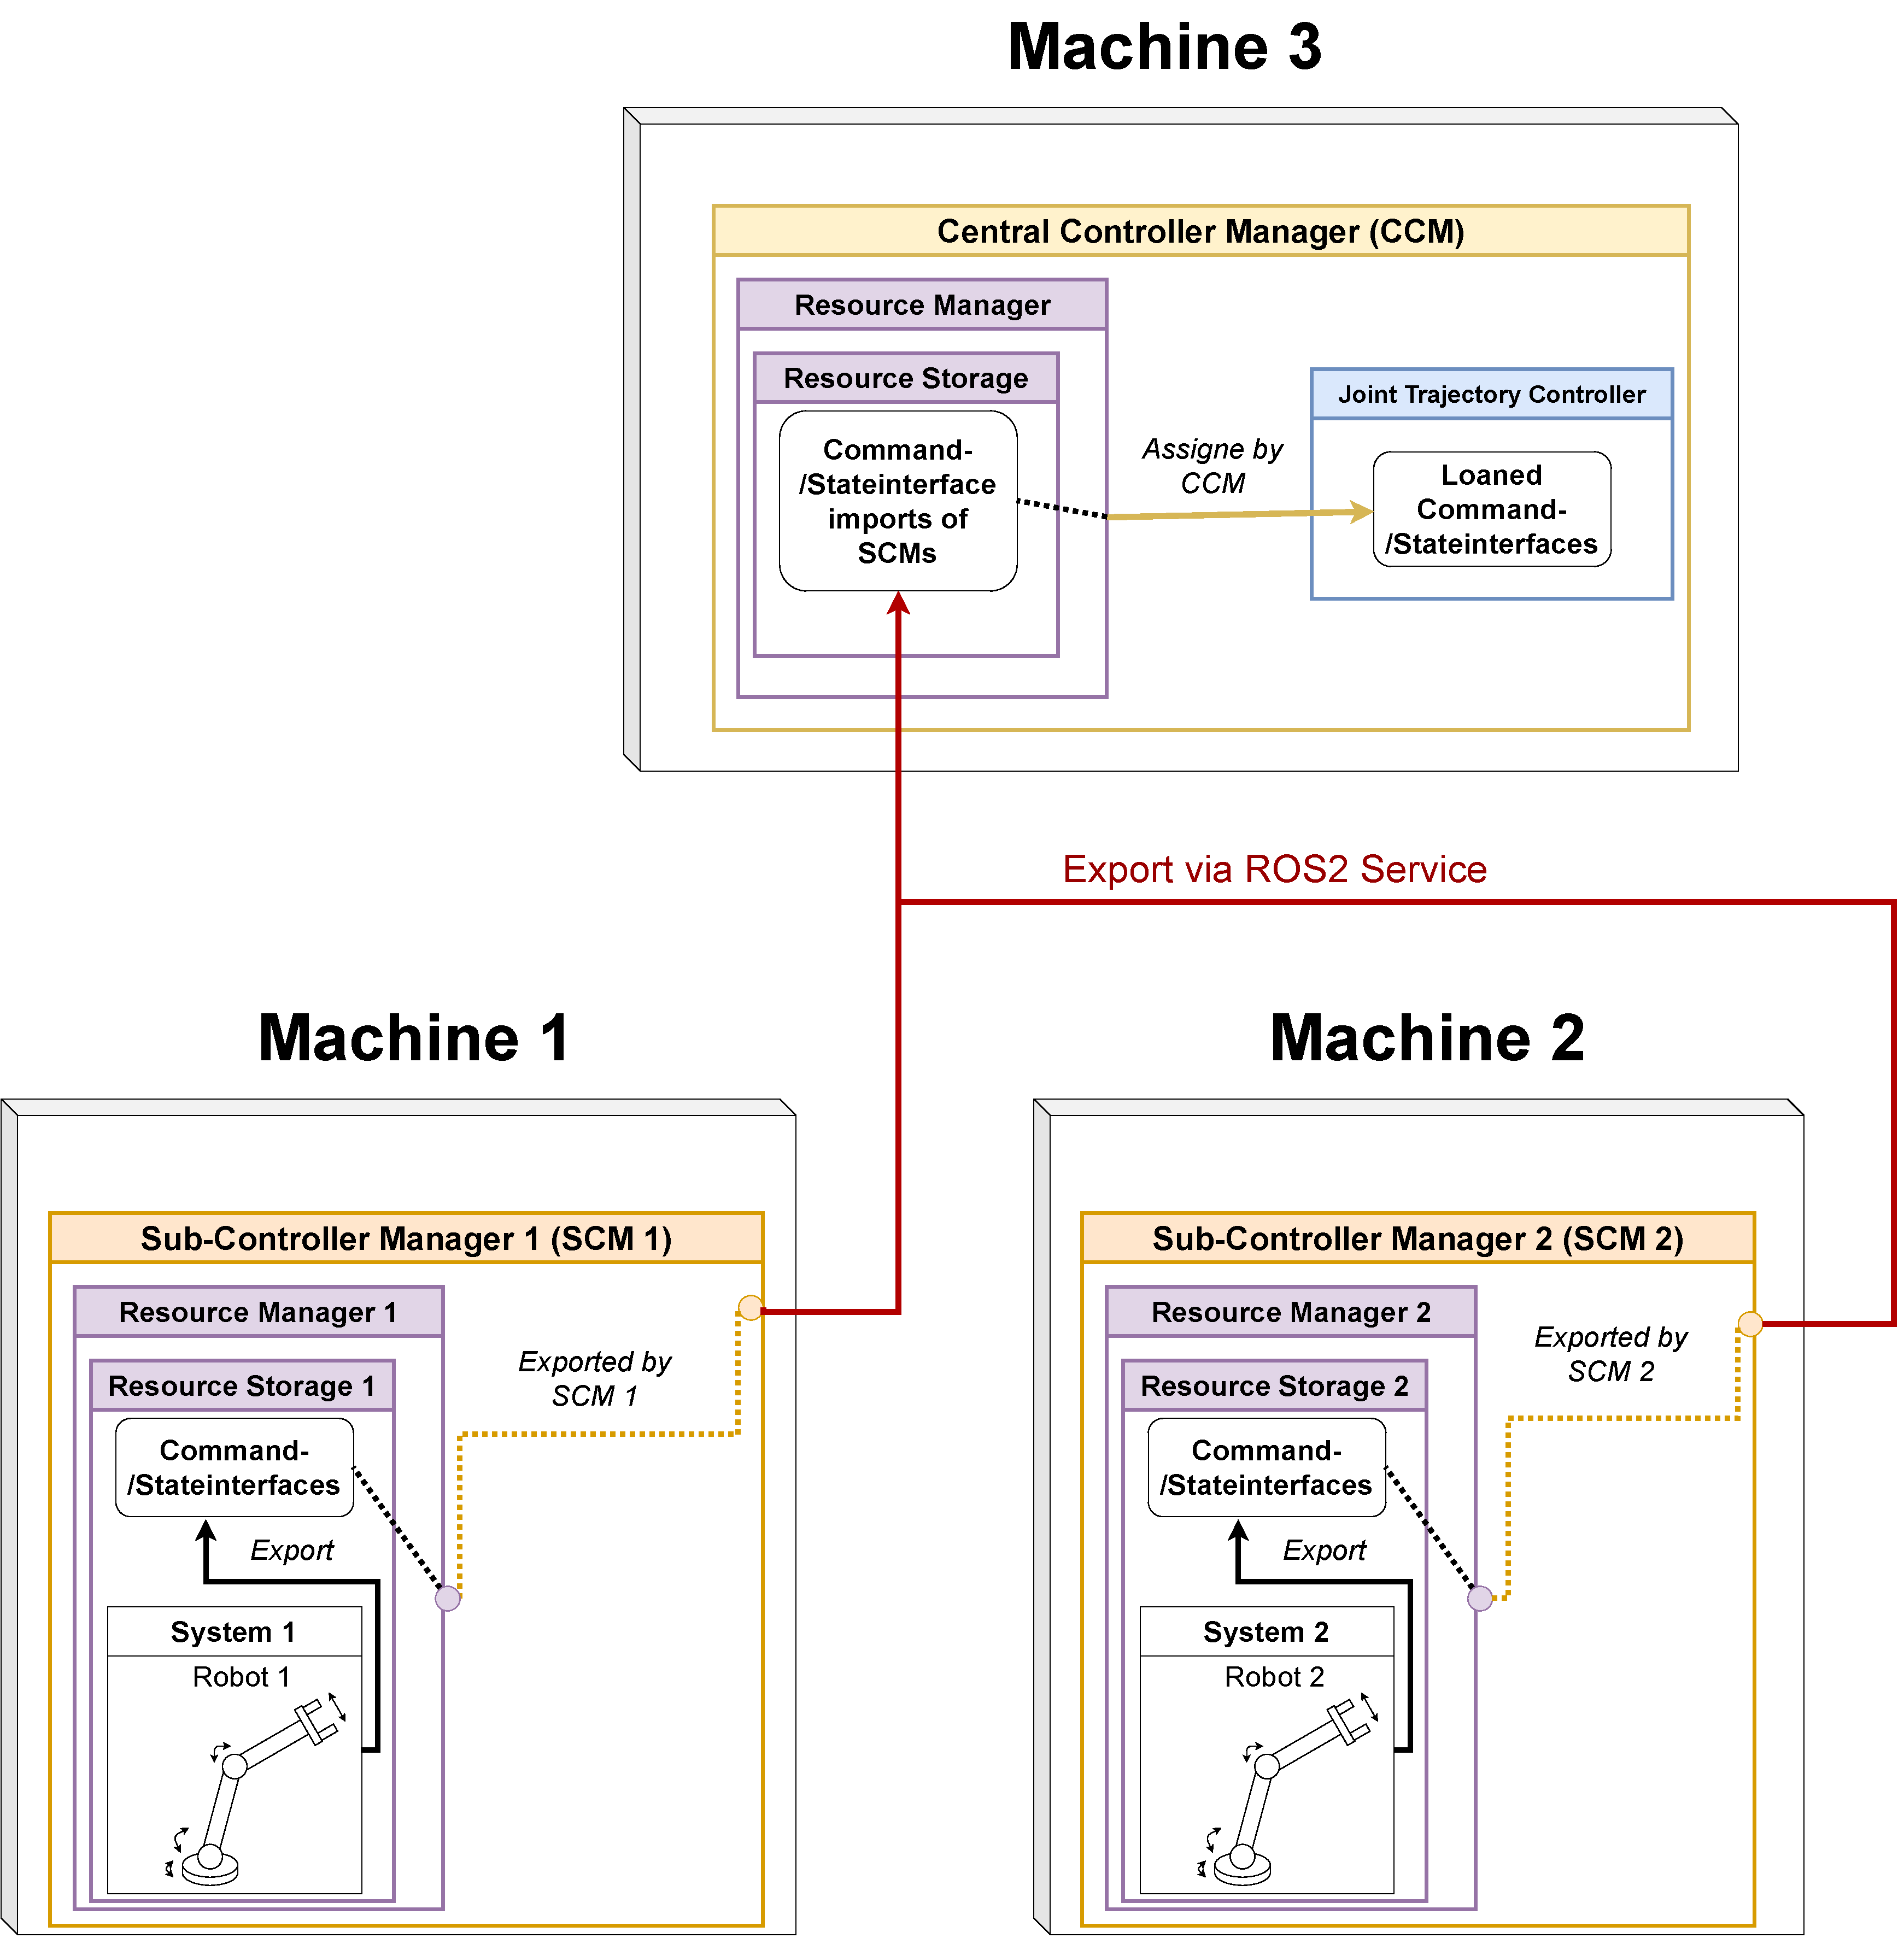
\includegraphics[width=1\textwidth]{Figures/c6/test_scenario_1.drawio.pdf}
	\caption{Schematic overview of the conceptual design of the system for the first test.}
	\label{c6_fig_test_scenario_1}
\end{figure}
\section{test 2}
\begin{figure}[htbp]
	\centering
	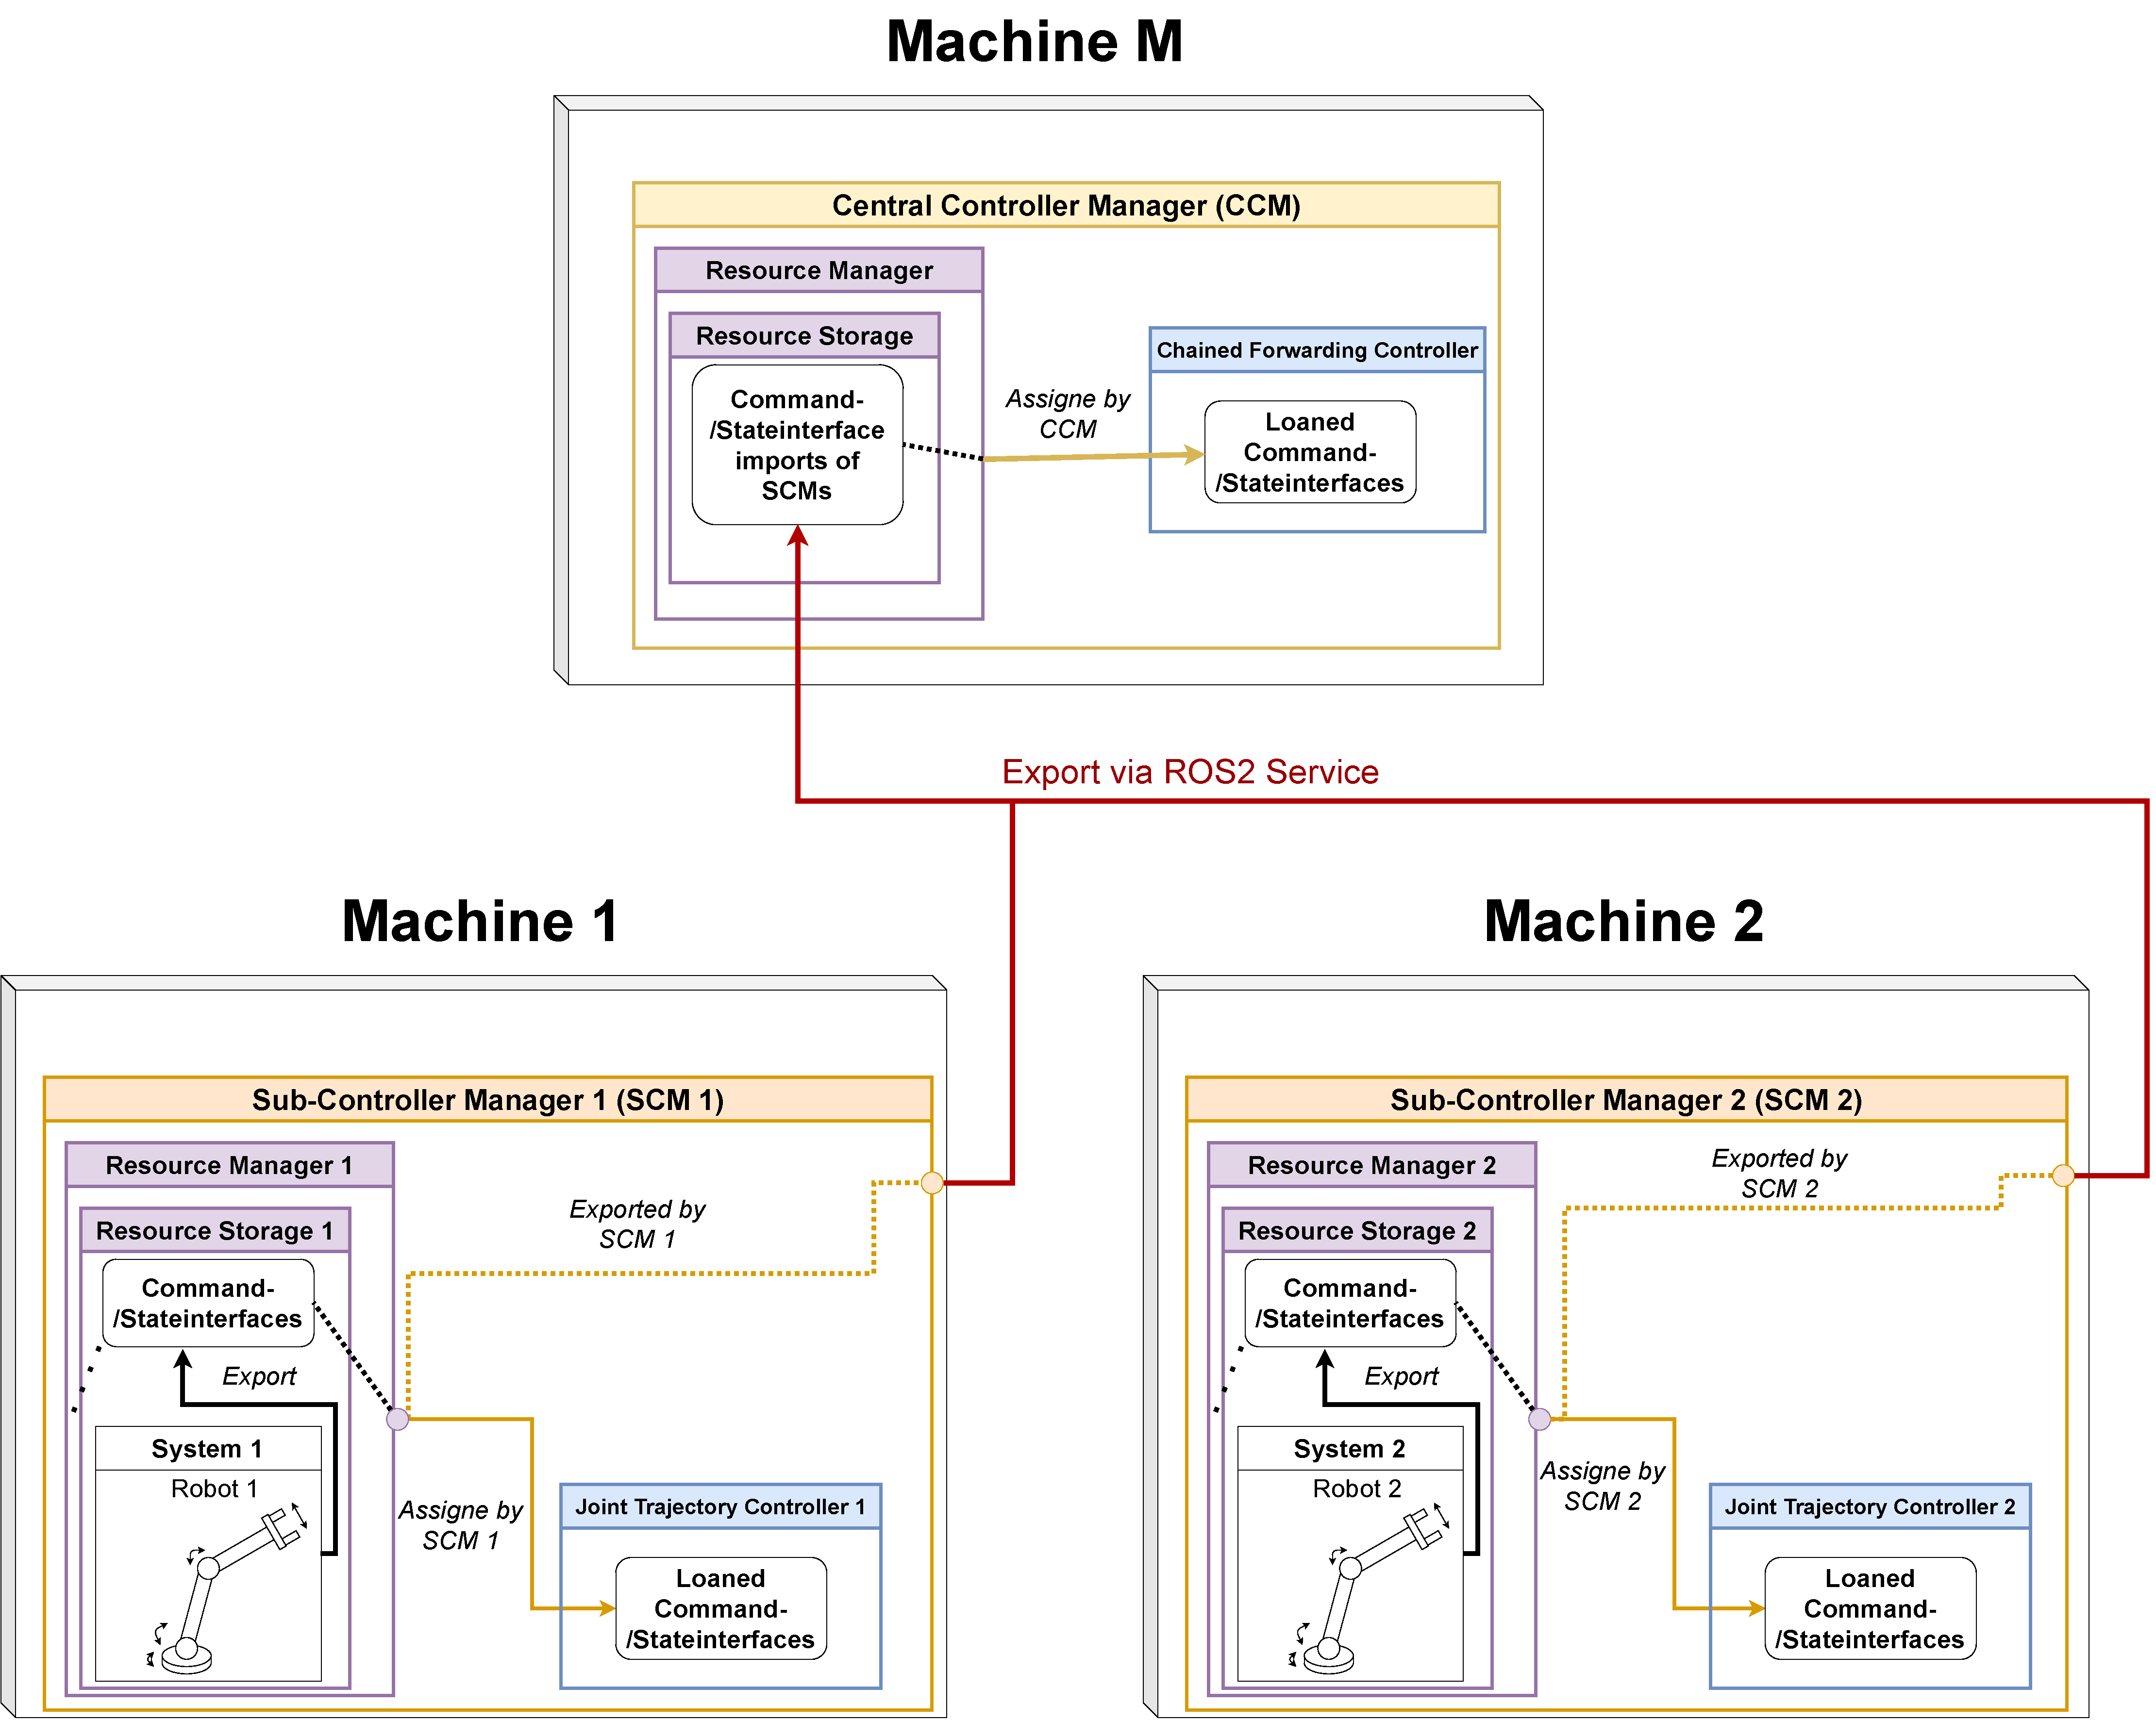
\includegraphics[width=1\textwidth]{Figures/c6/test_scenario_2.drawio.pdf}
	\caption{Schematic overview of the conceptual design of the system for the second test.}
	\label{c6_fig_test_scenario_2}
\end{figure}

\section*{Site Note}
Concept has also been tested on KUKA KR 16-2 KUKA KR 5 but because of how they are placed evaluation setup could not be conducted.
\missingfigure{Please add some figures}

